\newpage 
\section{Value at Risk (VaR)}

\subsection{Risk Measures}
\begin{definition}[Risk measure]
    A \textbf{risk measure} is a mapping that assigns a value $V_X$ to a given \textbf{payoff} random variable $X$.
\end{definition}

\noindent\newline These are a few examples of risk measures:
\begin{itemize}
    \item The \textbf{expected value premium principle} : 
    \begin{align*}
        V_X=\mathbb{E}[X] + \alpha\mathbb{E}[X]
    \end{align*}
    \noindent For some $\alpha\ge0$. For $\alpha=0$, $V_X=\mathbb{E}[X]$ is called the \textbf{pure premium risk measure}.

    \item The \textbf{standard deviation premium principle} : 
    \begin{align*}
        V_X = \mathbb{E}[X] - \alpha\sqrt{Var(X)}
    \end{align*}
    \noindent For some $\alpha\ge0$.

    \item The \textbf{Conditional Tail Expectation (CTE)} over negative payoff $X$ is defined as followed:
    \begin{align*}
        CTE_X = \mathbb{E}\Big[ X|X<0 \Big] = \frac{\mathbb{E}[X\1{X<0}]}{P(X<0)}
    \end{align*}
\end{itemize}

\begin{definition}[Coherent risk measure]
    A risk measure $V$ is said to be \textbf{coherent} if it satisfies the following properties:
    \begin{itemize}
        \item \textbf{Monotonicity : } $X \le Y\implies V_X \le V_Y$.
        \item \textbf{Positive Homogeneity : } $V_{\lambda X} = \lambda V_X, \lambda > 0$.
        \item \textbf{Translation invariance : } $V_{\mu + X} = \mu + V_X$.
        \item \textbf{Sub-additivity : } $V_{X+Y} \le V_X + V_Y$.
    \end{itemize}
\end{definition}

\begin{definition}[Distortion risk measure]
    A \textbf{distortion risk measure} is any risk measure of the form:
    \begin{align*}
        M_X = \mathbb{E}\Big[ Xg_X(X) \Big]
    \end{align*}

    \noindent Where $g_X$ is \textbf{non-negative, non-decreasing} function satisfying:
    \begin{itemize}
        \item $\mathbb{E}\Big[ g_X(X) \Big] = 1$.
        \item \textbf{Positive homogeneity : } $g_{\lambda X}(\lambda x) = g_X(x), \ \lambda > 0$.
        \item \textbf{Translation invariance : } $g_{X + \mu}(x+\mu) = g_X(x)$.
    \end{itemize}

    \noindent\newline The distortion risk measure $M_X$ satisfies the following properties:
    \begin{itemize}
        \item \textbf{Positive homogeneity : } For $\lambda > 0$, we have
        \begin{align*}
            \mathbb{E}\Big[ \lambda X g_{\lambda X}(\lambda X)\Big] = \mathbb{E}\Big[ \lambda X g_{X}(X)\Big] = \lambda \mathbb{E}\Big[ Xg_X(X) \Big]
        \end{align*}

        \item \textbf{Translation invariance : } For $\mu \ge 0$, we have
        \begin{align*}
            \mathbb{E}\Big[ (X + \mu)g_{X+\mu}(X+\mu) \Big] = \mathbb{E}\Big[ (X + \mu)g_{X}(X) \Big] = \mathbb{E}\Big[ Xg_X(X) \Big] + \mu\mathbb{E}\Big[ g_{X}(X) \Big] = \mathbb{E}\Big[ Xg_X(X) \Big] + \mu
        \end{align*}
    \end{itemize}
\end{definition}

\subsection{Quantile Risk Measures}
\subsubsection{Cumulative Distribution Function}
\begin{definition}[Cumulative Distribution Function (CDF)]
    The CDF of a random variable $X$ is defined as a function $F_X:\mathbb{R} \to [0,1]$ defined by:
    \begin{align*}
        F_X(x) = P(X \le x), \ \ x \ge 0
    \end{align*}
    \noindent Any CDF satisfies the following properties:
    \begin{itemize}
        \item \textbf{Non-decreasing}.
        \item \textbf{Right-continuous}.
        \item \textbf{$\lim_{x\to\infty F_X(x) = 1}$}.
        \item \textbf{$\lim_{x\to-\infty F_X(x) = 0}$}.
    \end{itemize}
\end{definition}

\noindent (The following are fundamental results of the CDFs, the proof will not be provided).
\begin{proposition}{Continuity of CDFs}{cont_of_cdf}
    For any non-decreasing sequence $(x_n)_{n\ge 1}$ such that $x_n \to x\in\mathbb{R}$, we have:
    \begin{align*}
        \lim_{n\to\infty}F_X(x_n) = \lim_{n\to\infty} P(X \le x_n) = P(X < x)
    \end{align*}
\end{proposition}

\begin{proposition}{Discontinuity of CDFs}{discont_of_cdf}
    The CDF of a random variable $X$ is right-continuous (not both way continuous). Hence, when there is a case where the CDF is discontinuous (figure \ref{fig:cdf-with-discont}) at a given point $x\in\mathbb{R}$, we can compute the probability that $X=x$:
    \begin{align*}
        P(X=x) = P(X\le x) - P(X < x) = F_X(x) - \lim_{y\to x^-}F_X(y)
    \end{align*}
\end{proposition}

\begin{figure}[ht]
    \centering
    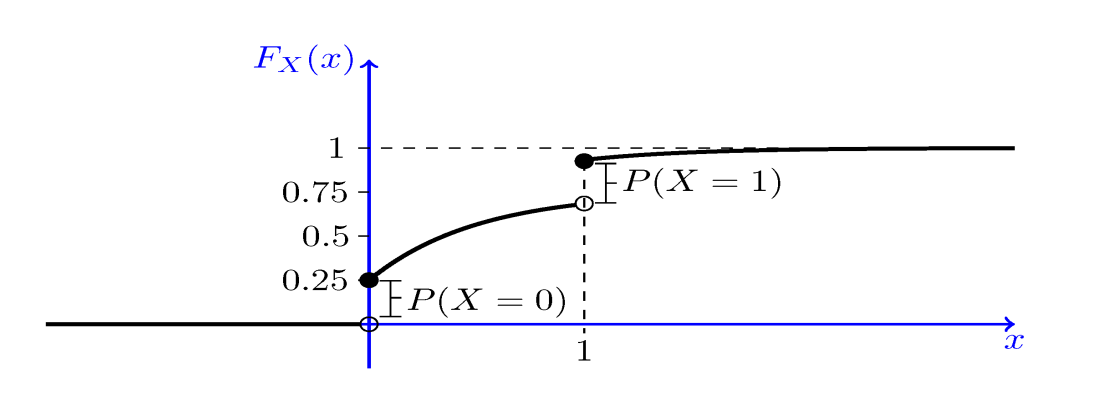
\includegraphics[width=\textwidth]{figures/cdf_with_discont.png}
    \caption{CDF with discontinuity (figure sampled from \cite{book:privault})}
    \label{fig:cdf-with-discont}
\end{figure}

\begin{definition}[Quantile]
    Given a random variable $X$ with the CDF $F_X:\mathbb{R}\to[0,1]$ and a level $p\in(0,1)$. The $p$-quantile of $X$ is given by:
    \begin{align*}
        q_X^p = \inf\Big\{x\in\mathbb{R} : F_X(x) \ge p\Big\}
    \end{align*}
\end{definition}

\noindent\newline \textbf{Remark} : Note that by proposition \ref{prop:discont_of_cdf}, we have:
    $P(X = q_X^p) = F_X(q_X^p) - \lim_{y \to (q_X^p)^-}F_X(y)$. Hence, when there is no discontinuity in $q_X^p$ ($P(X = q_X^p)=0$), we have :
\begin{align*}
    \boxed{
    P(X= q_X^p)=0 \implies p = \lim_{y \to (q_X^p)^-}F_X(y) = F_X(q_X^p)    
    }
\end{align*}

\subsubsection{Empirial Cumulative Distribution Function}
\begin{definition}[Empirical Cumulative Distribution Function (E-CDF)]
    The \textbf{Empirical Cumulative Distribution Function (E-CDF)} of an $N$-point dataset $\{x_1, \dots, x_N\}$ is estimated as:
    \begin{align*}
        F_N(x) = \frac{1}{N}\sum_{n=1}^N \1{x_n \le x}, \ \ x\ge0
    \end{align*}
\end{definition}

\subsection{Value at Risk (VaR)}
\begin{definition}[Value at Risk (VaR)]
    The \textbf{Value at Risk (VaR)} of a random variable $X$ at level $p\in(0,1)$ is the $p$-quantile of $X$:
    \begin{align*}
        \boxed{
            V_X^p = q_X^p = \inf\Big\{
                x \in \mathbb{R} : F_X(x) \ge p
            \Big\}
        }
    \end{align*}
\end{definition}

\begin{proposition}{Properties of Value at Risk}{properties_of_var}
    The Value at Risk (VaR) has the following properties:
    \begin{itemize}
        \item $(i)$ The function $p\to V_X^p$ is \textbf{non-decreasing, left-continuous} and it \textbf{admits limit from the right}.
        \item $(ii) \ V_X^p \le x \iff p\le P(X\le x)$.
        \item $(iii) \ V_{-X}^p = -V_X^{1-p}$.
    \end{itemize}
\end{proposition}

\begin{proof*}[Proposition \ref{prop:properties_of_var}]
    Proving each property, we have:
    \begin{subproof}{\newline Claim : $p\to V_X^p$ is non-decreasing, left-continuous and admits limit from the right}
        The function $p\to V_X^p$ (called the quantile function) is the \textbf{generalized inverse} of the Cumulative Distribution Function.

        \noindent\newline By proposition 2.3 - \cite{article:Embrechts2013}, since $F_X(x)$ is non-decreasing, the generalized inverse of it is non-decreasing, left-continuous and admits limits on the right.
    \end{subproof}

    \begin{subproof}{\newline Claim : $V_X^p \le x \iff p\le P(X\le x)$}
        Trivial due to the definition of Value at Risk (VaR).
    \end{subproof}

    \begin{subproof}{\newline Claim : $V_{-X}^p = -V_X^{1-p}$}
        We have:
        \begin{align*}
            F_{-X}(x) &= P(-X \le x) = P(X \ge -x) \\
                &= 1 - P(X < -x) = 1 - P(X \le -x) \\
                &= 1 - F_X(-x)
        \end{align*}

        \noindent Hence, we have:
        \begin{align*}
            p = F_{-X}(F_{-X}^{-1}(p)) = 1 - F_X(-F_{-X}^{-1}(p))
        \end{align*}
        \noindent Which yields:
        \begin{align}
            V_{-X}^p = F_{-X}^{-1}(p) = -F_{-X}^{-1}(1-p) = -V_X^{1-p}
        \end{align}
    \end{subproof}
\end{proof*}

\begin{theorem}{Coherence of Value at Risk (VaR)}{coherence_of_var}
    Value at Risk (VaR) satisfies:
    \begin{itemize}
        \item $(i)$ Monotonicity.
        \item $(ii)$ Positive homogeneity and translation invariance.
        \item $(iii)$ \textbf{But NOT} sub-additivity.
    \end{itemize}
\end{theorem}

\begin{proof*}[Theorem \ref{thm:coherence_of_var}]
    
\end{proof*}
    

\begin{definition}[Gaussian Value at Risk (G-VaR)]
    Given $X\sim \mathcal{N}(\mu_X, \sigma_X^2)$, we have:
    \begin{align*}
        \boxed{
            V_X^p = \mu_X + \sigma_X q_Z^p
        }
    \end{align*}
    \noindent Where the normal quantile $q_Z^p = V_Z^p$ at level $p$ satisfies:
    \begin{align*}
        \Phi(q_Z^p) = P(Z \le q_Z^p) = p, \ \ Z \sim \mathcal{N}(0,1)
    \end{align*}
    \noindent Meaning, we have:
    \begin{align*}
        V_X^p = \mu_X + \sigma_X \Phi^{-1}(p)
    \end{align*}
\end{definition}

\begin{lemma}{$X=V_X^U, P(U \ge p) \ne P(V_X^U \ge V_X^p)$}{x_equal_vx_power_u}
    We can write any random variable $X$ as:
    \begin{align*}
        X = V_X^U, \ U \sim Uniform(0,1)
    \end{align*}

    \noindent However, for any $p\in(0,1)$, we do not always have $P(U \ge p) = P(V_X^U \ge V_X^p)$. Instead, we have the following relationship:
    \begin{align*}
        P(V_X^U \ge V_X^p) &= P((V_X^U \ge V_X^p) \cap (U \ge p)) + P((V_X^U \ge V_X^p) \cap (U < p)) \\
        \text{Or : } P(X \ge V_X^p) &= P((X \ge V_X^p) \cap (U \ge p)) + P((X \ge V_X^p) \cap (U < p))
    \end{align*}

    \noindent This implies that the event $(V_X^U \ge V_X^p) \cap (U < p)$ can indeed have non-zero probability measure and it happens when there are discontinuities.
\end{lemma}

\begin{proof*}[Lemma \ref{lem:x_equal_vx_power_u}]
    By proposition \ref{prop:properties_of_var}, we have $P(V_X^p\le x) \iff p \le P(X\le x)$. Hence:
    \begin{align*}
        P(V_X^U \le x) &= P(U \le P(X\le x)) = P(X\le x) = F_X(x)
    \end{align*}
    \noindent To prove the second point, we have the following visual representation in figure \ref{fig:lemma3.1_illustration}.
    \begin{figure}[ht]
        \centering
        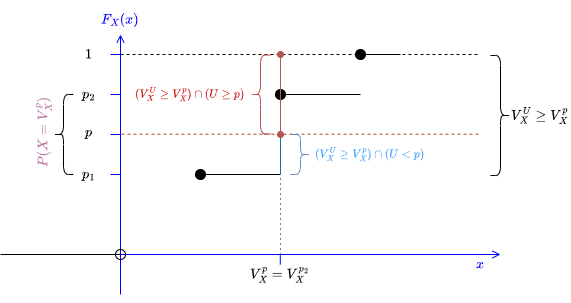
\includegraphics[width=\textwidth]{figures/lemma3.1-illustration.png}
        \caption{$P(V_X^U \ge V_X^p) = P((V_X^U \ge V_X^p) \cap (U \ge p)) + P((V_X^U \ge V_X^p) \cap (U < p))$}
        \label{fig:lemma3.1_illustration}
    \end{figure}
\end{proof*}

\begin{proposition}{Discontinuity at $V_X^p$}{discont_at_var}
    Let $V_X^p$ be the Value at Risk of a random variable $X$ at level $p\in(0,1)$. Then, we have:
    \begin{align*}
        P(X = V_X^p) = 0 \iff p = F_X(V_X^p) = \lim_{y\to x^-}F_X(y)
    \end{align*}

    \noindent\newline In other words, if there is no discontinuity at $V_X^p$, then $p = F_X(V_X^p)$.
\end{proposition}

\begin{proof*}[Proposition \ref{prop:discont_at_var}]
    By proposition \ref{prop:discont_of_cdf}, we have that when $P(X=V_X^p)=0$, we have $F_X(V_X^p) = P(X < V_X^p) = \lim_{y\to x^- F_X(y)}$. Now, we have to prove that $p=F_X(V_X^p)$. 

    \noindent\newline We have:
    \begin{align*}
        F_X(V_X^p) &= P(X \le V_X^p) = 1 - P(X > V_X^p) \\
        &= 1 - P(X \ge V_X^p) = 1 - P(V_X^U \ge V_X^p) \\
        &= 1 - P(U \ge p) \\
        &= 1 - (1 - p) = p
    \end{align*}

    \noindent\newline \textbf{Remark} : Note that by the visual representation in figure \ref{fig:lemma3.1_illustration}, when $P(X=V_X^p)=0$, we have:
    \begin{align*}
        P(V_X^U \ge V_X^p) = P(V_X^U \ge V_X^p \cap (U \ge p)) = P(U\ge p) 
    \end{align*}
\end{proof*}
